\documentclass[12pt, a4paper, english]{book}

% --- 1. Dil və Şrift Ayarları ---
\usepackage[T1]{fontenc}
\usepackage[utf8]{inputenc}
\usepackage[english]{babel}

% --- 2. Font + AMS Paketləri (ÇAKIŞMASIZ SIRA) ---
\usepackage{newtxtext}
\usepackage{newtxmath}
\let\Bbbk\relax
\let\openbox\relax
\usepackage{amsmath, amsfonts, amsthm}

% --- 3. Əsas Paketlər ---
\usepackage{thmtools}
\usepackage{mathtools}
\usepackage{indentfirst}
\usepackage{float}
\usepackage{tikz}
\usetikzlibrary{patterns}
\usetikzlibrary{arrows.meta}
\usepackage{pgfplots}
\pgfplotsset{compat=1.18}
\usepgfplotslibrary{fillbetween}
\usepackage{graphicx}
\usepackage{wrapfig}
\usepackage{enumitem}

% --- Venn Diaqramı Stili ---
\tikzset{
    Vennn pattern/.style={
        pattern=north east lines,
        pattern color=black!90,
        line width=0.6pt
    }
}

% --- 4. Səhifə Ölçüləri və Header ---
\usepackage[top=2cm, bottom=2cm, left=2cm, right=2cm, headheight=15pt, headsep=1cm]{geometry}
\usepackage{fancyhdr}
\pagestyle{fancy}
\fancyhf{}
\fancyhead[L]{\nouppercase{\leftmark}}
\fancyhead[R]{\nouppercase{\rightmark}}
\fancyfoot[C]{\thepage}

\fancypagestyle{plain}{
  \fancyhf{}
  \fancyfoot[C]{\thepage}
  \renewcommand{\headrulewidth}{0pt}
}

% --- 5. Nömrələmə Strukturu ---
\renewcommand{\thepart}{\Roman{part}}
\renewcommand{\thechapter}{\Roman{chapter}}
\renewcommand{\thesection}{\arabic{section}}
\renewcommand{\thesubsection}{\thesection.\arabic{subsection}}
\renewcommand{\thesubsubsection}{\thesubsection.\arabic{subsubsection}}
\numberwithin{figure}{section}
\numberwithin{equation}{section}

% --- 6. Teorem Stilləri ---
\newtheoremstyle{springerth}
  {10pt}{10pt}{\itshape}{}{\bfseries}{.}{.5em}{}
\theoremstyle{springerth}
\newtheorem{theorem}{Theorem}[section]
\newtheorem{lemma}[theorem]{Lemma}

\newtheoremstyle{springerdef}
  {10pt}{10pt}{\normalfont}{}{\bfseries}{.}{.5em}{}
\theoremstyle{springerdef}
\newtheorem{definition}{Definition}[section]
\newtheorem{example}{Example}[section]
\newtheorem{exercise}{Exercise}[section]
\newtheorem*{example*}{Example}

\renewcommand{\proofname}{\bfseries Proof}

% --- 7. mdframed Mühitləri ---
\usepackage[framemethod=TikZ]{mdframed}

\newmdenv[
    topline=true, bottomline=true, leftline=false, rightline=false,
    linewidth=1.5pt, linecolor=black!80,
    skipabove=20pt, skipbelow=20pt,
    innertopmargin=10pt, innerbottommargin=10pt,
    font={\small\itshape},
    frametitle={\large\textit{\textbf{Note:}}},
    nobreak=true
]{academicnote}

\newenvironment{scientist}[2]{
    \vspace{25pt}
    \begin{mdframed}[
        hidealllines=true, nobreak=true,
        innertopmargin=20pt, innerbottommargin=20pt,
        singleextra={
            \draw[line width=0.8pt] (P) -- (P-|O) node[pos=0, circle, fill=black, inner sep=1.8pt]{} node[pos=1, circle, fill=black, inner sep=1.8pt]{};
            \node[fill=white, inner sep=5pt] at ([xshift=0.5\textwidth]P-|O) {\Large $\cdot \ \infty \ \cdot$};
            \draw[line width=0.8pt] (O) -- (O-|P) node[pos=0, circle, fill=black, inner sep=1.8pt]{} node[pos=1, circle, fill=black, inner sep=1.8pt]{};
            \node[fill=white, inner sep=5pt] at ([xshift=0.5\textwidth]O-|P) {\Large $\cdot \ \infty \ \cdot$};
        }
    ]
    \begin{center}
        \small \textbf{\textsc{Historical Note: #1}}
    \end{center}
    \vspace{10pt}
    \begin{wrapfigure}{l}{0.25\textwidth}
        \vspace{-15pt}
        \centering
        \includegraphics[width=\linewidth]{#2}
        \vspace{-20pt}
    \end{wrapfigure}
    \itshape \noindent \ignorespaces
}{
    \par \end{mdframed} \vspace{20pt}
}

\newmdenv[
    topline=false, bottomline=false, rightline=false, leftline=true,
    linewidth=1.5pt, linecolor=black!40,
    backgroundcolor=white,
    skipabove=12pt, skipbelow=12pt,
    innerleftmargin=15pt, innerrightmargin=10pt,
    innertopmargin=5pt, innerbottommargin=5pt,
    font={\small\itshape},
    frametitle={\large\textbf{\textit{Meaning:}}},
    frametitlefont={\small\bfseries\upshape},
    frametitleaboveskip=0pt,
    nobreak=true
]{logicbox}

\newmdenv[
    topline=false, bottomline=false, rightline=false, leftline=true,
    linewidth=3pt, linecolor=black!90,
    backgroundcolor=gray!5,
    skipabove=15pt, skipbelow=15pt,
    innertopmargin=10pt, innerbottommargin=10pt,
    innerleftmargin=12pt,
    font={\small},
    frametitle={\large\textit{\textbf{Attention:}}},
    frametitlefont=\small\bfseries\upshape,
    nobreak=true
]{important}

% --- 8. Referans və Linklər ---
\usepackage{hyperref}
\hypersetup{hidelinks}
\usepackage[english]{cleveref}
\usepackage[symbol]{footmisc}

\crefname{figure}{figure}{figures}
\Crefname{figure}{Figure}{Figures}
\crefname{equation}{equation}{equations}
\Crefname{equation}{Equation}{Equations}
\crefname{theorem}{theorem}{theorems}
\Crefname{theorem}{Theorem}{Theorems}
\crefname{definition}{definition}{definitions}
\Crefname{definition}{Definition}{Definitions}
\crefname{section}{section}{sections}
\Crefname{section}{Section}{Sections}

\addto\captionsenglish{%
  \renewcommand{\figurename}{Figure}%
  \renewcommand{\tablename}{Table}%
}

\begin{document}

\section{Construction of the set of natural numbers}
Let us build, using Peano's axioms, the set of \textbf{natural numbers} $\mathbb{N}$.

\begin{itemize}
\item \textbf{Reflexivity}: $a=a$.
\item \textbf{Symmetry}: $a=b \iff b=a$.
\end{itemize}

\begin{enumerate}[leftmargin=2cm, align=left]
    \item[Axiom 1.] $1$ is a natural number, i.e. $1\in\mathbb{N}$.
    \item[Axiom 2.] For every $x\in\mathbb{N}$ there exists a unique successor $A(x)$.\footnotemark[1]
    \item[Axiom 5 (Induction).] If $1\in S$ and $A(x)\in S$ for every $x\in S$, then $S=\mathbb{N}$.
\end{enumerate}

\footnotetext[1]{This axiom lets us construct all other natural numbers: $A(1)=2$, $A(2)=3$, and so on.}

\begin{important}
To prove $X(n)$ holds for every $n \in \mathbb{N}$: check the base case $n=1$, then prove $X(n) \implies X(n+1)$.
\end{important}

\begin{academicnote}
The Hindu-Arabic decimal positional system we use today was developed in \textbf{India}, later replacing Roman numerals in Europe.
\end{academicnote}

\begin{logicbox}
$S = \{ y \in \mathbb{N} \mid x + y \text{ is well-defined} \}$ collects every $y$ for which the claim holds.
\end{logicbox}

\subsection{Definition of addition}

\begin{theorem}[Existence and uniqueness of addition]
For every $x, y \in \mathbb{N}$ there exists a unique $x+y$ satisfying:
\begin{equation*}
    x + 1 = A(x), \qquad x + A(y) = A(x+y).
\end{equation*}
\end{theorem}

\begin{proof}
Fix $x$, let $S = \{ y \mid x+y \text{ unique}\}$. Base: $y=1$ gives $A(x)$, so $1\in S$. Step: if $y \in S$ then $A(x+y)=x+A(y)$, so $A(y)\in S$. By induction, $S=\mathbb{N}$.
\end{proof}

\begin{definition}[Sum]
The number $x+y$ above is called the \textbf{sum} of $x$ and $y$.
\end{definition}

\begin{theorem}
$$1+3=4$$
\end{theorem}

\begin{proof}
$$1+3 = 1+A(2) = A(1+2) = A(A(2)) = A(3) = 4.$$
\end{proof}

\begin{theorem}{Commutativity of addition:} $$x+y=y+x.$$
\end{theorem}

\begin{proof}
Follows by double induction, first fixing $x=1$, then applying the induction hypothesis on $x$.
\end{proof}

\begin{center}
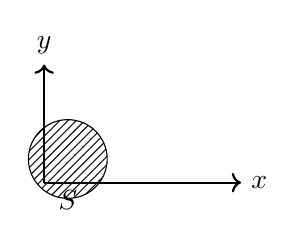
\begin{tikzpicture}
\draw[thick,->] (0,0) -- (2.5,0) node[right] {$x$};
\draw[thick,->] (0,0) -- (0,1.5) node[above] {$y$};
\fill[Vennn pattern] (0.3,0.3) circle (0.5);
\draw (0.3,0.3) circle (0.5) node[below=8pt] {$S$};
\end{tikzpicture}
\end{center}

\end{document}